\chapter{Alt Uzay ve Çarpım Topolojisi}

Alt uzay topolojisi bir uzayın alt kümesine miras kalan topolojiyi tanımlar.
Çarpım topolojisi ise iki uzayı birleştirerek yeni bir uzay kurar.

%-------------------------------------------------------------------
\section{Konu}

\begin{definition}[Alt Uzay Topolojisi]
$(X, \tau)$ uzayı ve $A \subseteq X$ verilsin. \textbf{Alt uzay topolojisi:}
\[
\tau_A = \{U \cap A : U \in \tau\}.
\]
\end{definition}

\begin{sezgi}
$A$'yı $X$'ten kesilen bir ``pencere'' gibi düşünün. $A$ üzerindeki açıkları
sıfırdan tanımlamayız; $X$'in hazır açıklarını $A$ ile keser, ne kadarı $A$'ya
düşüyorsa onu açık sayarız. Bu yüzden $\tau_A$, $\tau$'dan \emph{miras} alınır.
\end{sezgi}

\begin{figure}[ht]
\centering
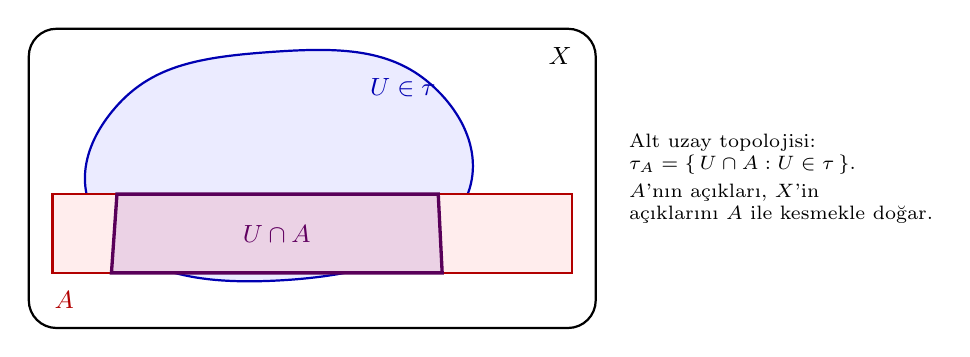
\begin{tikzpicture}[scale=1.0, font=\small]
  % Ambient space X
  \draw[rounded corners=10pt, thick] (-0.5,-1.6) rectangle (6.7,2.2);
  \node at (6.25,1.85) {$X$};
  % Open set U of X
  \draw[blue!70!black, thick, fill=blue!8]
    plot[smooth cycle, tension=0.8] coordinates
    {(0.5,-0.4) (2.6,-1.0) (4.9,-0.2) (4.6,1.5) (2.5,1.9) (0.6,1.2)};
  \node[blue!70!black] at (4.25,1.45) {$U \in \tau$};
  % Subset A (a horizontal strip)
  \draw[red!70!black, thick, fill=red!7]
    (-0.2,-0.9) rectangle (6.4,0.1);
  \node[red!70!black] at (-0.05,-1.25) {$A$};
  % Intersection U cap A highlighted
  \draw[violet!70!black, very thick, fill=violet!22, fill opacity=0.7]
    (0.55,-0.9) -- (4.75,-0.9) -- (4.7,0.1) -- (0.62,0.1) -- cycle;
  \node[violet!75!black, align=center] at (2.65,-0.4)
    {$U \cap A$};
  \node[align=left, anchor=west, font=\scriptsize] at (7.0,0.3)
    {Alt uzay topolojisi:\\ $\tau_A = \{\,U \cap A : U \in \tau\,\}$.\\[2pt]
     $A$'nın açıkları, $X$'in\\ açıklarını $A$ ile kesmekle doğar.};
\end{tikzpicture}

\caption{Alt uzay topolojisi: $A \subseteq X$'te açıklar $U \cap A$ biçimindedir.}
\end{figure}

\begin{definition}[Çarpım Topolojisi]
$(X, \tau_X)$ ve $(Y, \tau_Y)$ verilsin. Çarpım topolojisi $X \times Y$ üzerinde
$\{U \times V : U \in \tau_X,\, V \in \tau_Y\}$ bazından üretilir.
\end{definition}

Projeksiyon $\pi_X: X \times Y \to X$ ve $\pi_Y: X \times Y \to Y$ süreklidir.

\begin{sezgi}
Çarpım topolojisinin bazı, düzlemdeki açık dikdörtgenlere benzer: bir ``yatay''
açık $U$ ile bir ``dikey'' açık $V$'yi çarparak $U \times V$ kutusunu kurarız.
Bu kutular tüm açıkların \emph{bazıdır} --- açıklar bu kutuların birleşimleridir.
\end{sezgi}

\begin{figure}[ht]
\centering
\begin{tikzpicture}[scale=1.0, font=\small]
  % Axes for X (horizontal) and Y (vertical)
  \draw[-{Stealth}] (-0.3,0) -- (5.6,0) node[right] {$X$};
  \draw[-{Stealth}] (0,-0.3) -- (0,4.4) node[above] {$Y$};
  % U interval on X axis
  \draw[blue!70!black, very thick] (1.4,0) -- (3.8,0);
  \node[blue!70!black, below=2pt] at (2.6,0) {$U \in \tau_X$};
  % V interval on Y axis
  \draw[red!70!black, very thick] (0,1.3) -- (0,3.5);
  \node[red!70!black, left=2pt, rotate=90, anchor=south] at (0,2.4) {$V \in \tau_Y$};
  % Basic box U x V
  \draw[violet!70!black, thick, fill=violet!15]
    (1.4,1.3) rectangle (3.8,3.5);
  \node[violet!75!black] at (2.6,2.4) {$U \times V$};
  % Dashed guide lines
  \draw[blue!60!black, dashed] (1.4,0) -- (1.4,1.3);
  \draw[blue!60!black, dashed] (3.8,0) -- (3.8,1.3);
  \draw[red!60!black, dashed] (0,1.3) -- (1.4,1.3);
  \draw[red!60!black, dashed] (0,3.5) -- (1.4,3.5);
  \node[align=left, anchor=west, font=\scriptsize] at (4.4,3.4)
    {Çarpım topolojisinin\\ baz elemanı: bir\\ dikdörtgen kutu\\ $U \times V$.};
\end{tikzpicture}

\caption{Çarpım topolojisinin baz elemanı: $U \times V$ dikdörtgen kutusu.}
\end{figure}

\begin{figure}[ht]
\centering
\begin{tikzpicture}[scale=1.0, font=\small]
  % Product box X x Y in the middle-top
  \draw[violet!70!black, thick, fill=violet!10] (2.0,1.6) rectangle (5.2,3.6);
  \node[violet!75!black] at (3.6,3.9) {$X \times Y$};
  \fill (3.6,2.6) circle (1.8pt);
  \node[font=\scriptsize, above right=0pt] at (3.6,2.6) {$(x,y)$};
  % X line bottom-left
  \draw[blue!70!black, thick, fill=blue!8] (-0.4,-0.4) rectangle (2.6,0.4);
  \node[blue!70!black] at (2.3,0.55) {$X$};
  \fill (1.1,0.0) circle (1.8pt) node[below=2pt, font=\scriptsize] {$x$};
  % Y line bottom-right
  \draw[red!70!black, thick, fill=red!8] (4.6,-0.4) rectangle (7.6,0.4);
  \node[red!70!black] at (4.9,0.55) {$Y$};
  \fill (6.1,0.0) circle (1.8pt) node[below=2pt, font=\scriptsize] {$y$};
  % projection arrows
  \draw[blue!70!black, -{Stealth}, thick]
    (3.2,1.5) to[bend right=18] node[left, font=\scriptsize, pos=0.55] {$\pi_X$} (1.0,0.55);
  \draw[red!70!black, -{Stealth}, thick]
    (4.2,1.5) to[bend left=18] node[right, font=\scriptsize, pos=0.55] {$\pi_Y$} (6.2,0.55);
  \node[font=\scriptsize, align=center] at (3.6,-1.15)
    {$\pi_X(x,y)=x,\quad \pi_Y(x,y)=y$ \; (her ikisi sürekli)};
\end{tikzpicture}

\caption{$\pi_X$ ve $\pi_Y$ projeksiyonları $(x,y)$ noktasını bileşenlerine düşürür.}
\end{figure}

\begin{karsiornek}
``$U \times V$ biçiminde olmayan açık yok'' demek yanlıştır. Birim diskte
$D(0,1) \times D(0,1)$ içindeki dairesel bir bölge, hiçbir tek $U \times V$
kutusuna eşit olmasa da açıktır; çünkü açıklar kutuların \emph{birleşimidir}.
$\{U \times V\}$ yalnızca \textbf{baz}'dır, topolojinin tamamı değil.
\end{karsiornek}

\begin{table}[h]
\centering
\begin{tabular}{lll}
\toprule
\textbf{Özellik} & \textbf{Alt uzay} & \textbf{Çarpım} \\
\midrule
Hausdorff & \checkmark & \checkmark \\
Kompaktlık & Yalnız kapalı alt uzay & \checkmark (Tychonoff) \\
Bağlantılılık & Hayır (genel) & \checkmark \\
T0/T1/T2 & \checkmark & \checkmark \\
\bottomrule
\end{tabular}
\caption{Topolojik özelliklerin kalıtımı}
\end{table}

%-------------------------------------------------------------------
\section{Teoremler}

\begin{theorem}
Hausdorff uzayın her alt uzayı Hausdorff'tur.
\begin{proof}[İspat eskizi]
$x \ne y$ noktaları $A \subseteq X$ içinde olsun. $X$ Hausdorff olduğundan
$X$'te ayrık açıklar $U \ni x$, $V \ni y$ vardır. O hâlde $U \cap A$ ve
$V \cap A$, $A$'da açık, $x$ ile $y$'yi ayıran komşuluklardır ve
$(U \cap A) \cap (V \cap A) = (U \cap V) \cap A = \emptyset$.
\end{proof}
\end{theorem}

\begin{theorem}
Kompakt uzayın kapalı alt uzayı kompakttır.
\begin{proof}[İspat eskizi]
$A \subseteq X$ kapalı, $X$ kompakt olsun. $A$'nın bir açık örtüsü
$\{U_\alpha \cap A\}$ verilsin. Her $U_\alpha$'yı açık olan $X \setminus A$ ile
birlikte alırsak $X$'in açık örtüsünü elde ederiz; $X$ kompakt olduğundan
sonlu alt-örtü vardır. $X \setminus A$'yı atınca $A$'yı örten sonlu sayıda
$U_\alpha \cap A$ kalır.
\end{proof}
\end{theorem}

\begin{theorem}
$X$ ve $Y$ bağlantılı $\Rightarrow X \times Y$ bağlantılıdır.
\begin{proof}[Kanıt İskeleti]
$\{x_0\} \times Y$ ve $X \times \{y_0\}$ bağlantılı dilimler; kesişimleri üzerinden birleşerek tüm çarpımı kapsar.
\end{proof}
\end{theorem}

\begin{theorem}[Tychonoff, $n=2$]
$X$ ve $Y$ kompakt $\Rightarrow X \times Y$ kompakttır.
\end{theorem}

\begin{theorem}
$X$ ve $Y$ Hausdorff $\Rightarrow X \times Y$ Hausdorff'tur.
\begin{proof}[İspat eskizi]
$(x_1,y_1) \ne (x_2,y_2)$ ise $x_1 \ne x_2$ veya $y_1 \ne y_2$. Diyelim
$x_1 \ne x_2$; $X$'te ayrık $U_1 \ni x_1$, $U_2 \ni x_2$ seçilir. O zaman
$U_1 \times Y$ ve $U_2 \times Y$ çarpımda açık, ayrık ve iki noktayı ayırır.
\end{proof}
\end{theorem}

\begin{theorem}[Evrensel Özellik — Çarpım]
$f: Z \to X \times Y$ sürekli $\Leftrightarrow \pi_X \circ f$ ve $\pi_Y \circ f$ süreklidir.
\begin{proof}[İspat eskizi]
($\Rightarrow$) Projeksiyonlar sürekli, sürekli fonksiyonların bileşkesi
süreklidir. ($\Leftarrow$) Bir baz elemanı $U \times V$'nin ön-görüntüsü
$f^{-1}(U \times V) = (\pi_X \circ f)^{-1}(U) \cap (\pi_Y \circ f)^{-1}(V)$
olup iki açık ön-görüntünün kesişimi olarak $Z$'de açıktır; baz üzerinde
süreklilik tüm topolojide sürekliliği verir.
\end{proof}
\end{theorem}

%-------------------------------------------------------------------
\section{Algoritmalar}

\subsection{finite\_subspace — $O(|\tau| \cdot |A|)$}

\begin{algorithm}
\caption{Subspace$(X, \tau, A)$}
\begin{algorithmic}[1]
\State $\tau_A \leftarrow \{\}$
\For{each $U \in \tau$}
    \State $\tau_A$.add$(U \cap A)$
\EndFor
\State \Return $(A, \tau_A)$
\end{algorithmic}
\end{algorithm}

\subsection{binary\_product — $O(|\tau_X| \cdot |\tau_Y|)$}

\begin{algorithm}
\caption{Product$(X, \tau_X, Y, \tau_Y)$}
\begin{algorithmic}[1]
\State basis $\leftarrow \{U \times V : U \in \tau_X,\, V \in \tau_Y\}$
\State \Return topology\_from\_basis$(X \times Y,$ basis$)$
\end{algorithmic}
\end{algorithm}

%-------------------------------------------------------------------
\section{pytop API}

\begin{lstlisting}[language=Python]
from pytop import (
    finite_subspace,
    binary_product,
    sierpinski_space,
    discrete_topology,
    indiscrete_topology,
    make_topology,
    make_set,
    empty_set,
    is_compact,
    is_connected,
    is_t2,
    separation_inherited_by_subspace,
)
\end{lstlisting}

\texttt{finite\_subspace(space, subset)} $\to$ \texttt{FiniteTopologicalSpace}

\texttt{binary\_product(left, right)} $\to$ \texttt{FiniteTopologicalSpace} (carrier: çift-demetler)

\texttt{separation\_inherited\_by\_subspace(subspace\_obj, feature="hausdorff")} $\to$ \texttt{Result}

%-------------------------------------------------------------------
\section{Örnekler}

\subsection*{Örnek 5.1 — Alt Uzay: Ayrık Topoloji}

\begin{lstlisting}[language=Python]
d4 = discrete_topology(1, 2, 3, 4)
sub12 = finite_subspace(d4, [1, 2])
print("carrier:", sub12.carrier)
print("topology:", sorted([sorted(list(u)) for u in sub12.topology],
                          key=lambda x: (len(x), x)))
\end{lstlisting}

\begin{verbatim}
carrier: (1, 2)
topology: [[], [1], [2], [1, 2]]
\end{verbatim}

\subsection*{Örnek 5.4 — Çarpım: $D(0,1) \times D(0,1)$}

\begin{lstlisting}[language=Python]
d2 = discrete_topology(0, 1)
prod_dd = binary_product(d2, d2)
print("carrier:", sorted(prod_dd.carrier))
print("topology size:", len(list(prod_dd.topology)))
print("compact:", is_compact(prod_dd).status)
print("connected:", is_connected(prod_dd).status)
\end{lstlisting}

\begin{verbatim}
carrier: [(0, 0), (0, 1), (1, 0), (1, 1)]
topology size: 16
compact: true
connected: false
\end{verbatim}

\subsection*{Örnek 5.5 — Çarpım: Sierpiński $\times$ Sierpiński}

\begin{lstlisting}[language=Python]
ss = binary_product(s, s)
print("topology size:", len(list(ss.topology)))
print("compact:", is_compact(ss).status)
print("connected:", is_connected(ss).status)
\end{lstlisting}

\begin{verbatim}
topology size: 6
compact: true
connected: true
\end{verbatim}

\subsection*{Örnek 5.7 — İndiscrete'in Alt Uzayı İndiscrete'tir}

\begin{lstlisting}[language=Python]
ind4 = indiscrete_topology(1, 2, 3, 4)
sub_ind = finite_subspace(ind4, [1, 2])
print("carrier:", sub_ind.carrier)
print("topology:", sorted([sorted(list(u)) for u in sub_ind.topology],
                          key=lambda x: (len(x), x)))
print("connected:", is_connected(sub_ind).status)
\end{lstlisting}

\begin{verbatim}
carrier: (1, 2)
topology: [[], [1, 2]]
connected: true
\end{verbatim}

\subsection*{Örnek 5.8 — Hausdorff Kalıtımı ve Çarpıma Etkisi}

\begin{lstlisting}[language=Python]
d4 = discrete_topology(1, 2, 3, 4)
sub_d = finite_subspace(d4, [1, 2])
inh = separation_inherited_by_subspace(sub_d, "hausdorff")
print("subspace Hausdorff inherited:", inh.status)

prod_T2 = binary_product(d2, d2)
print("D(0,1) x D(0,1) T2:", is_t2(prod_T2).status)
prod_notT2 = binary_product(d2, indiscrete_topology(0, 1))
print("D(0,1) x Ind(0,1) T2:", is_t2(prod_notT2).status)
\end{lstlisting}

\begin{verbatim}
subspace Hausdorff inherited: true
D(0,1) x D(0,1) T2: true
D(0,1) x Ind(0,1) T2: false
\end{verbatim}

%-------------------------------------------------------------------
\section{Alıştırmalar}

\subsection*{Kodlama}

\begin{enumerate}[label=K\arabic*.]
\item Sierpiński uzayının $\{0\}$ ve $\{1\}$ alt uzaylarını oluşturun ve
      hangi topolojiyi taşıdığını belirleyin.
\item 4-noktalı özel bir uzayda $\{2,3\}$ alt uzayını bulun.
\item \texttt{binary\_product(sierpinski\_space(), discrete\_topology(0,1))}
      için \texttt{is\_compact} ve \texttt{is\_connected} kontrol edin.
\item \texttt{indiscrete\_topology(1,2,3,4)} uzayının \texttt{[1,2]} alt uzayını
      oluşturup açık küme sayısı ile \texttt{is\_connected} çıktısını bulun;
      Örnek~5.7 ile karşılaştırın.
\item \texttt{separation\_inherited\_by\_subspace} ile
      \texttt{discrete\_topology(1,2,3)}'ten alınan \texttt{[1,2]} alt uzayının
      Hausdorff özelliğini miras alıp almadığını kontrol edin.
\end{enumerate}

\subsection*{Teori}

\begin{enumerate}[label=T\arabic*.]
\item Alt uzay topolojisinde dahil etme $i: A \to X$'in sürekli olduğunu ispatlayın.
\item $X$ ve $Y$ bağlantılı $\Rightarrow X \times Y$ bağlantılı olduğunu ispatlayın.
\item Çarpımın evrensel özelliğini ispatlayın: $f: Z \to X \times Y$ sürekli
      $\Leftrightarrow \pi_X \circ f$ ve $\pi_Y \circ f$ süreklidir.
\end{enumerate}
